\section{Les applications possibles de l'intelligence artificielle au sein des ERP}

Maintenant que nous avons vu les applications possibles des principaux concepts de l'intelligence artificielle et les services devant être proposés par les ERP, nous pouvons réfléchir aux applications possibles de l'intelligence artificielle concernant les ERP.

\subsection{Gestionnaire Électronique des Documents}

Au sein d'un ERP, il est très courant de rencontrer un système de gestion électronique des documents, dont le rôle est de gérer les documents électroniques de la compagnie.
Nous avons d'ailleurs développé une GED au sein de \textsc{Sigma} au cours de mon apprentissage.

Il existe quatre étapes majeures dans la gestion électronique des documents~:~acquisition, traitement, stockage et diffusion.
\\
\begin{itemize}
    \item[\tiny$\bullet$] L'acquisition des documents au sein de la GED peut s'effectuer par l'intégration de documents préalablement scannés, ou par la production automatique de documents via un logiciel.
    \item[\tiny$\bullet$] Le traitement des documents consiste en leur indexation. C'est la description du document qui permettra de le retrouver facilement par la suite.
    \item[\tiny$\bullet$] Le stockage des documents doit être effectué sur un support prenant en compte le volume potentiel de documents que la GED devra gérer dans le futur, il doit être sécurisé de manière à garantir la sécurité des données.
    \item[\tiny$\bullet$] La diffusion des documents doit permettre aux utilisateurs de retrouver les documents dont ils ont besoin facilement et rapidement.
\end{itemize}
~\\

Différentes utilisations de l'intelligence artificielle peuvent intervenir lors de ces quatre étapes afin d'améliorer les capacités d'une GED.

\subsubsection{Classification de documents}

L'un des domaines dans lequel l'intelligence artificielle excelle et s'améliore rapidement de nos jours est la classification, que ce soit des documents, images, textes, mails, etc.

Dans une GED, avec une architecture et une organisation précise prédéfinie, il peut être intéressant d'utiliser un système permettant de classer les documents importés au bon endroit au sein de la structure sans que l'utilisateur n'ait besoin d'intervenir.
Afin de fonctionner correctement, un tel système nécessite de nombreuses données d'entraînement.
C'est grâce à ces dernières qu'il pourra apprendre à classifier correctement les documents au sein de l'architecture.
Un tel système ne peut donc être mis en place que sur une GED ayant été classée manuellement depuis un certain temps, afin d'avoir plusieurs exemplaires de chaque type de documents déjà classés au sein de l'architecture.

Il existe de nombreux concepts d'intelligence artificielle permettant de classifier des fichiers.
Les plus poussés sont actuellement les réseaux de neurones à convolution qui permettent de classifier des images avec des taux d'erreur extrêmement bas.
Cependant, nous voulons ici classifier des documents et nous allons voir que nous pouvons utiliser des concepts beaucoup plus basiques et requérant bien moins de puissance de calcul pour atteindre un résultat satisfaisant.

\paragraph*{Préparation des documents}
~\\

Pour classer un document, les êtres humains sont capables de repérer quasiment instantanément les détails permettant d'en identifier la nature exacte, que ce soit par la lecture de certains mots clés ou par le repérage d'un logo par exemple.
L'objectif ici est de trouver un concept d'intelligence artificielle qui soit capable de faire la même chose.

Il y a deux possibilités majeures sur la manière dont le système peut traiter des documents.
\\
\begin{itemize}
    \item[\tiny$\bullet$] La première serait de considérer les documents comme des images.
    Le principal avantage serait que si des documents sont principalement discernables de par leurs caractéristiques graphiques plus que de par leur contenu, le système serait capable de les classifier sans difficulté.
    Cependant, le cas inverse se présente également et comme nous traitons ici des documents généralement administratifs, il est plus courant que ces documents aient une charte graphique semblable et se discernent principalement de par leur contenu.
    En plus de cela, les documents n'ont pas toujours le même nombre de pages. Or il est très préférable que toutes les images à classifier aient les mêmes dimensions pour que ce genre de systèmes fonctionnent correctement.
    
    \item[\tiny$\bullet$] La seconde possibilité est de préalablement extraire le texte des documents afin de pouvoir se baser sur le contenu de ceux-ci pour les classer.
    Pour extraire le texte brut d'un document il existe de nombreuses méthodes d'OCR, en français reconnaissance optique de caractères, qui sont robustes et utilisables sur des pdf complets en une simple ligne de code~;~il n'est donc pas intéressant de les décrire plus que cela.
    Avant de donner tout le texte d'un document à un système de classification, il est cependant nécessaire d'effectuer des traitements permettant d'en extraire des <<~features~>>, <<~caractéristiques~>> en français.
    C'est sur ces caractéristiques que le système pourra se baser afin de classer les documents.
    Une démarche intéressante serait par exemple d'utiliser la méthode de pondération TF-IDF (term frequency-inverse document frequency).
    Celle-ci est très utilisée en fouille de textes, car elle permet de mesurer l'importance de chaque terme employé dans un texte.
    Avec cette méthode on pourrait, par exemple, extraire les cinq termes les plus importants dans le document et utiliser uniquement ces cinq termes afin de classer ce dernier.
\end{itemize}
~\\

Dans notre cas, la meilleure solution serait sans doute d'utiliser la seconde méthode, consistant en l'extraction des principales caractéristiques directement depuis le texte de chaque document.
Avec cette méthode on peut donc générer une base de données reliant les termes les plus importants avec chaque document dont ils sont extraits.
Ainsi, nous posséderions une base de données avec tous les documents déjà présents dans la GED, ces données serviraient de données d'entraînement au système de classification.
Une fois le système entraîné, lorsqu'un nouveau document sera importé, il suffira d'en extraire les caractéristiques et de les envoyer dans le système pour que le document soit classé automatiquement.

\paragraph*{Algorithmes de classification}
~\\

Une fois les données prêtent, nous pouvons analyser les documents en comparant le nombre de termes en communs parmi leurs caractéristiques extraites.
C'est pour effectuer cette comparaison que l'algorithme de classification va entrer en jeu.
Sachant que les caractéristiques extraites ne seront pas très nombreuses on peut utiliser des classifieurs linéaires relativement basiques, tels que les SVM (<<~support vector machine~>> traduit par <<~machine à vecteurs de support~>>),  la classification naïve bayésienne, ou même la méthode des $k$ plus proches voisins.

Les trois méthodes précédemment citées sont des concepts de base de l'intelligence artificielle qui sont enseignés en tant qu'introduction dans beaucoup de cours, portants sur l'intelligence artificielle.
Cependant, cela ne signifie pas qu'ils sont inutiles ou inefficients~;~ils sont au contraire, simple à développer et à appliquer, et peuvent être utilisés lorsque la situation s'y prête.
Comme déjà précisé, nous nous basons sur un nombre de caractéristiques très limité pour cette classification.
Ces classifieurs sont donc adaptés à notre cas de figure avec des avantages et inconvénients pour chacun d'entre eux.
\\
\begin{itemize}
    \item[\tiny$\bullet$] Le principe des machines à vecteurs de support (séparateurs à vaste marge) est de placer des frontières entre les catégories.
    On peut en visualiser le fonctionnement facilement si on prend un exemple simple de classification ne contenant que deux classes.
    Considérons les données suivantes, dans lesquelles les deux classes sont <<~ronds~>> et <<~triangles~>> et la donnée que l'on veut classer dans une de ces dernières est le carré rouge.
    
    \FloatBarrier
    \begin{figure}[h!]
        \begin{minipage}[c]{0.5\textwidth}
            \begin{center}
                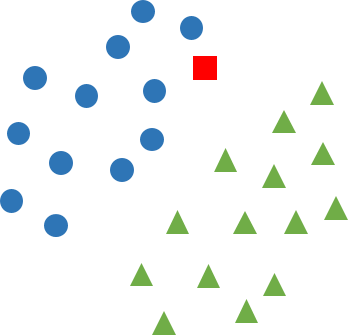
\includegraphics[width = 0.35\textwidth]{svm_1}
            \end{center}
        \end{minipage}\hfill
        \begin{minipage}[c]{0.5\textwidth}
            \caption{Problème de classification en deux dimensions}
            \label{figure:svm_1}
        \end{minipage}
    \end{figure}
    \FloatBarrier
    
    En tant qu'être humain, il est trivial de déterminer que le carré devrait être classé avec les ronds, au vu de l'organisation présente.
    C'est cependant nettement plus complexe pour une machine.
    Le but du SVM va être de déterminer une droite <<~frontière~>> qui permette de séparer les données en deux classes.
    Le SVM choisit une frontière qui maximise la marge, c'est-à-dire qu'elle est le plus éloignée possible des deux classes.
    Cela permettra de classer avec plus de précision les futures données inconnues.
    
    Par exemple, dans la figure ci-dessous on voit deux frontières noires en pointillés qui permettent de classifier correctement les données d'entraînement.
    En revanche elles ne maximisent pas la marge entre les deux classes, ce qui peut donner lieu à de mauvaises classifications dans le futur.
    La frontière maximisant la marge, qui sera donc déterminée par le SVM, est symbolisée en rouge.

    \FloatBarrier
    \begin{figure}[h!]
        \begin{minipage}[c]{0.5\textwidth}
            \begin{center}
                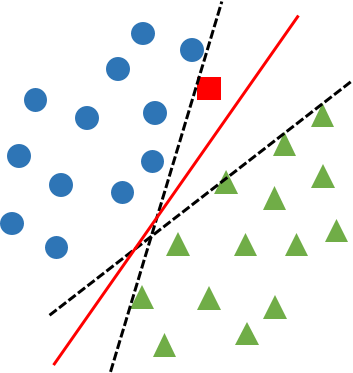
\includegraphics[width = 0.35\textwidth]{svm_2}
            \end{center}
        \end{minipage}\hfill
        \begin{minipage}[c]{0.5\textwidth}
            \caption{Détermination de la frontière maximisant la marge par le SVM}
            \label{figure:svm_2}
        \end{minipage}
    \end{figure}
    \FloatBarrier
    
    Les SVM peuvent classifier des données avec plus de deux dimensions, ils s'appliquent donc correctement à notre cas.
    
    Avant de pouvoir utiliser un SVM pour classer des données il faut déjà que celui-ci soit entraîné.
    Cet entraînement s'effectue grâce aux données déjà présentent au sein de la GED (plus le nombre de classes et de caractéristiques sera élevé et plus le temps et les besoins en puissance de calcul augmenteront).
    Cela signifie que pour entraîner un SVM il faut utiliser une machine assez performante.
    Dans notre cas, le nombre de classes de documents et de caractéristiques utilisées devrait rester assez limité pour qu'une machine récente soit capable de réaliser cette tâche.
    L'avantage est que, une fois l'entraînement du SVM effectué, il peut être utilisé sur un ordinateur extrêmement peu puissant afin de classer de nouvelles données.
    Les utilisateurs de la GED pourront donc utiliser n'importe quel type de matériel.
    ~\\
    
    \item[\tiny$\bullet$] La classification naïve bayésienne est basée sur le théorème de \textsc{Bayes} et utilise des formules de statistiques.
    
    Le théorème de \textsc{Bayes} est le suivant~:~
    $$P(h|d) = \frac{(P(d|h) \cdot P(h))}{P(d)}$$
    Où~:~
    \begin{itemize}
        \item[\tiny$-$] $P(h|d)$, est la probabilité de l'hypothèse $h$ sachant la donnée $d$.
        \item[\tiny$-$] $P(d|h)$, est la probabilité de la donnée $d$ sachant que l'hypothèse $h$ est vraie.
        \item[\tiny$-$] $P(h)$, est la probabilité que l'hypothèse $h$ soit vraie.
        \item[\tiny$-$] $P(d)$, est la probabilité de la donnée $d$.
    \end{itemize}
    Dans notre cas, nous voulons calculer toutes les probabilités du type \textit{P(caractéristique$|$classe de document)}.
    Par exemple, la probabilité \textit{P(livraison$|$bon de livraison)} sera élevée puisque le terme <<~livraison~>> sera une caractéristique forte des documents de classe <<~bon de livraison~>>, tandis que \textit{P(facture$|$bon de livraison)} sera basse.
    
    On calcule ainsi toutes les probabilités d'apparition des caractéristiques pour chaque classe.
    Ensuite lorsque nous voulons classer un nouveau document il suffit d'extraire ses caractéristiques et d'observer les probabilités du type P(classe$|$caractéristique) et la plus haute donnera la classe du document.
    ~\\
    
    \item[\tiny$\bullet$] La méthode des $k$ plus proches voisins est une méthode qui à l'avantage d'être plutôt intuitive et donc simple à comprendre et implémenter.
    Le but est ici de comparer les caractéristiques du nouveau document avec les caractéristiques de tous les documents déjà présents dans la GED.
    Une fois cette comparaison effectuée, le document le plus <<~proche~>> du nouveau est celui qui aura le plus de caractéristiques en commun avec lui.
    Le nouveau document est classé dans la même classe que le voisin le plus proche.
    
    L'explication ci-dessus ne prend en compte qu'un seul voisin le plus proche.
    Cependant pour de meilleures performances il peut être intéressant de sélectionner, par exemple, les cinq voisins les plus proches et attribuer au nouveau document la classe apparaissant le plus souvent parmi ces derniers.
    Le nombre de voisins considérés correspond à la variable $k$.
    Il est préférable de toujours choisir une valeur de $k$ impaire afin de toujours pouvoir déterminer une classe sans souci.
    
    Le principal désavantage de cette méthode est qu'elle ne possède pas de phase d'apprentissage à proprement parler.
    À la place la totalité des échantillons présents dans la base sont parcourus à chaque ajout de nouveau document.
    Cela est fortement contraignant, car plus le nombre de documents présents dans la GED sera grand, plus le processus de classification des nouveaux sera long.
    Cela signifie aussi que les utilisateurs de la GED doivent posséder un ordinateur capable d'une puissance de calcul suffisante pour classer chaque nouveau document.
\end{itemize}
~\\

Pour choisir une méthode de classification parmi les trois proposées ci-dessus, il faut analyser leurs défauts et avantages.
En termes de puissance de calcul nécessaire, le choix se portera sans nul doute sur la classification naïve bayésienne.
Celle-ci nécessite juste le calcul d'un nombre fortement limité de probabilités que n'importe quelle machine peut assumer, la classification des nouvelles données se fait ensuite instantanément.
En revanche, le SVM n'est un choix valable qu'en possession d'une machine permettant son entraînement.
La méthode des $k$ plus proches voisins est, quant à elle, peu envisageable, sachant qu'elle nécessite que tous les utilisateurs possèdent une machine puissante, de plus, son processus de classification est lent.

Afin d'aller plus loin, et d'éventuellement améliorer la précision de la classification, on peut imaginer un système se basant à la fois sur des caractéristiques provenant du texte et d'autres provenant de la charte graphique du document.

\subsubsection{Partitionnement de documents}

Il y a un type d'apprentissage que nous n'avons pas encore abordé, l'apprentissage non supervisé.
Le principe pour le système utilisant ce type d'apprentissage est de tenter de trouver des structures sous-jacentes à partir de données non étiquetées.
Dans notre cas, les données non étiquetées correspondent aux documents bruts, non classés.

Un apprentissage non supervisé doit permettre de mettre en évidence des caractéristiques communes à des données, afin de les organiser par groupes ne contenant que des données similaires.

Dans notre cas, un système de partitionnement des documents pourrait être utile pour organiser automatiquement les documents.
Un avantage est que ces systèmes nécessitent des données qui n'ont pas préalablement été classées.

Les systèmes de partitionnement de documents sont beaucoup utilisés pour les moteurs de recherches.
En effet, il est courant d'obtenir des milliers de pages de résultats pour une requête et le partitionnement des résultats en catégories permet de déterminer ceux qui sont le plus susceptibles d'intéresser l'utilisateur.
Dans notre cas on pourrait par exemple imaginer un système de recherche de documents au sein de la GED qui permette de trier les documents sur les classes générées par le système.
On pourrait même utiliser un système de partitionnement de documents en plus d'un système de classification et ainsi effectuer un partitionnement sur les factures qui permettrait de les regrouper automatiquement par clients, etc.
Le partitionnement de documents pourrait donc s'employer à l'importation de nouveaux documents ainsi que durant les recherches avancées des utilisateurs.
Les utilisations possibles sont multiples.

Afin d'effectuer un partitionnement sur des documents, il est nécessaire de faire certaines préparations préalables.
Au même titre que pour la classification il faut nettoyer le texte de la ponctuation et des <<~mots vides~>>, avant d'appliquer la méthode TF-IDF abordée plus tôt, ou une méthode comparable.
On peut ensuite commencer le processus de partitionnement sur les caractéristiques ainsi extraites.

Des recherches sont en cours dans le domaine du partitionnement afin d'y appliquer des méthodes d'apprentissage profond, mais nous allons ici voir des méthodes plus courantes.
Il existe actuellement quatre catégories d'algorithmes de partitionnement de données.

\paragraph*{Le partitionnement en \textit{k}-moyennes}
~\\

Cette méthode permet de partitionner des données en $k$ groupes, de façon à minimiser la fonction de distance entre les données d'un même groupe.

Pour cette méthode il est nécessaire de choisir à l'avance la valeur de $k$ qui détermine le nombre de groupes.
Lorsque le nombre de groupes voulus est déjà connu, il suffit de renseigner $k$ en conséquence, mais lorsque ce n'est pas le cas il faut appliquer une méthode pour le déterminer.

La méthode généralement appliquée est la <<~elbow method~>>, la méthode du coude.
Elle consiste à tracer une courbe exprimant les valeurs de $k$ testées en fonction de la variance obtenue.
La variance se calcule en divisant la variance entre les groupes par la variance entre toutes les données.
La courbe ainsi obtenue forme un coude et c'est la valeur $k$ en ce point qu'il faut choisir.

Le principal désavantage est que pour déterminer la meilleure valeur de $k$ il faut exécuter l'algorithme pour toutes les valeurs testées.
Un second désavantage est que la méthode définit toujours les groupes avec des tailles similaires, même si cela n'est pas adapté à la situation, comme on peut le voir ci-dessous, le groupe vert devrait être plus important que les bleus et rouges.

\FloatBarrier
\begin{figure}[h!]
    \begin{minipage}[c]{0.45\textwidth}
        \begin{center}
            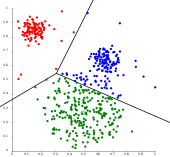
\includegraphics[width = 0.5\textwidth]{k_means}
        \end{center}
    \end{minipage}\hfill
    \begin{minipage}[c]{0.45\textwidth}
        \caption{Partitionnement de données en appliquant la méthode des \textit{k}-moyennes}
        \label{figure:k_means}
    \end{minipage}
\end{figure}
\FloatBarrier

Cette méthode fait partie des méthodes de base qui sont enseignées pour la facilité de leur mise en place, mais les cas d'utilisations en situations réelles sont plutôt rares.

\paragraph*{Le regroupement hiérarchique}
~\\

Les méthodes de regroupement hiérarchique présentent l'avantage de ne pas avoir besoin de déterminer à l'avance le nombre de groupes à créer.
Un autre avantage est qu'elles permettent une visualisation de la hiérarchie créée via un dendrogramme, qui est un type de diagramme.

Le but étant de placer chaque document existant au sein de l'architecture, il y a deux approches possibles~:~par agglomération ou par division.
\\
\begin{itemize}
    \item[\tiny$\bullet$] L'approche par agglomération consiste à initialement considérer chaque document comme un groupe à part entière.
    Ces derniers sont ensuite regroupés par leurs caractéristiques communes les plus proches jusqu'à ne former qu'un seul groupe.
    \item[\tiny$\bullet$] L'approche par division est l'exact opposé, on débute avec un seul groupe englobant la totalité des données.
    Ensuite, on sépare les données en groupes de plus en plus petits en fonction des caractéristiques, jusqu'à ce que tous les documents soient séparés dans des groupes individuels.
\end{itemize}
~\\

Ces méthodes permettent de générer une architecture hiérarchique que l'on peut facilement visualiser.

Ce type de regroupement est fortement efficace sur des données possédant des relations hiérarchiques fortes entre elles.
Les documents stockés au sein d'une GED ne possèdent pas forcément de lien hiérarchique, par conséquent, ce type de regroupement n'est peut-être pas l'idéal pour notre cas de figure.

\paragraph*{Le partitionnement basé sur les lois de probabilités}
~\\

Ce modèle est basé sur des lois de probabilités.
Les groupes sont définis comme des objets appartenant à une même distribution de probabilité.

Ce type de partitionnement diffère des autres de par le fait qu'ici tous les éléments font partie de chaque groupe, mais avec un degré d'appartenance différent.
Par exemple, sur l'image ci-dessous on peut voir que les points bleus font partie du groupe rouge, cependant leur degré d'appartenance au groupe bleu est plus fort.

\FloatBarrier
\begin{figure}[h!]
    \begin{minipage}[c]{0.45\textwidth}
        \begin{center}
            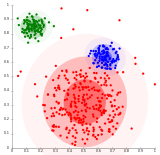
\includegraphics[width = 0.5\textwidth]{distribution}
        \end{center}
    \end{minipage}\hfill
    \begin{minipage}[c]{0.45\textwidth}
        \caption{Visualisation d'un partitionnement effectué en utilisant la loi de probabilité normale}
        \label{figure:distribution}
    \end{minipage}
\end{figure}
\FloatBarrier

Cette méthode est généralement combinée avec la méthode des $k$-moyennes, car il est nécessaire de déterminer préalablement le nombre $k$ de groupes à former.
Cependant, les deux méthodes combinées permettent de donner de très bons résultats.

\paragraph*{Le partitionnement sur la densité}
~\\

L'algorithme le plus populaire de cette catégorie est le DBSCAN (density-based spatial clustering of applications with noise), il se base sur les zones présentant une densité de points supérieure au reste de l'espace des données, pour les regrouper par groupes.

Cet algorithme permet de déterminer par lui-même le nombre de groupes à trouve.
Il est capable de gérer les données aberrantes et ainsi est très peu sensible au bruit.
C'est cette dernière raison qui en fait un algorithme autant utilisé dans le domaine.
En revanche, il ne permet pas une définition précise des bords de chaque groupe, car il est courant que la densité des points soit moins haute à ces endroits.

\paragraph*{Conclusion}
~\\

Aucune méthode de partitionnement de données ne donne de résultats parfaits, mais il est important de noter que les applications de ces méthodes ne nécessitent généralement pas un partitionnement précis.

Selon le cas de figure, il peut être intéressant d'utiliser soit la méthode de partitionnement utilisant les distributions de probabilité, soit celle utilisant la densité.

La première garantie que toutes les données appartiennent à un groupe.
Il peut donc être intéressant de l'utiliser à l'importation d'un nouveau document au sein de la GED afin de garantir qu'il soit classé dans un groupe.

Si l'on souhaite plutôt appliquer une méthode de partitionnement au moment d'une recherche par un utilisateur il peut être intéressant d'utiliser le partitionnement basé sur la densité.
Puisque dans ce cas on souhaite diriger l'utilisateur vers les documents les plus susceptibles de l'intéresser.

\subsubsection{Extraction de données pour saisie automatique}

Il est très courant que des employés aient besoin de saisir dans un système informatique des informations qu'ils ont devant eux, sous format papier ou numérique.
Cependant, il existe des méthodes qui peuvent permettre d'automatiser la saisie de ces données simplement en important un fichier au sein du système.

La compagnie \textsc{Rossum}, fondée en 2017, a créé l'outil ELIS.
L'utilisation de cet outil est simple, on y importe une facture et l'outil est capable d'analyser automatiquement la structure de celle-ci afin d'extraire les informations utiles et de les ajouter directement au sein d'une base de données.
Afin de rester compétitive, l'entreprise ne dévoile pas le fonctionnement de son logiciel, mais il est intéressant d'imaginer les méthodes d'intelligence artificielle employées.

Cette section est dédiée à la conception d'un système, inspiré d'ELIS, qui serait capable de gérer plusieurs types de documents.

Les différentes étapes au sein de ce système seraient les suivantes.
\\
\begin{enumerate}
    \item Détection automatique du type de document. Si la nature du document est mal déterminée, l'outil permet à l'utilisateur de le corriger. Après une correction de la part d'un utilisateur le système apprend de son erreur afin de continuellement s'adapter aux nouveaux documents importés.
    
    \item Analyse de la structure du document. Ici l'outil annote sur le document les zones correspondantes aux informations à récupérer. L'utilisateur peut le corriger, ce qui permet encore une fois un apprentissage à partir des erreurs.
    
    \item Application d'une méthode de reconnaissance de caractères afin de lire les informations présentent dans les zones délimitées à l'étape précédente.
    
    \item Enregistrement des informations directement en base de données.
\end{enumerate}
~\\

On peut voir ci-dessous un aperçu du fonctionnement de l'outil ELIS qui relie chaque champ à la zone du document détectée comme correspondante.

\FloatBarrier
\begin{figure}[h!]
    \begin{center}
        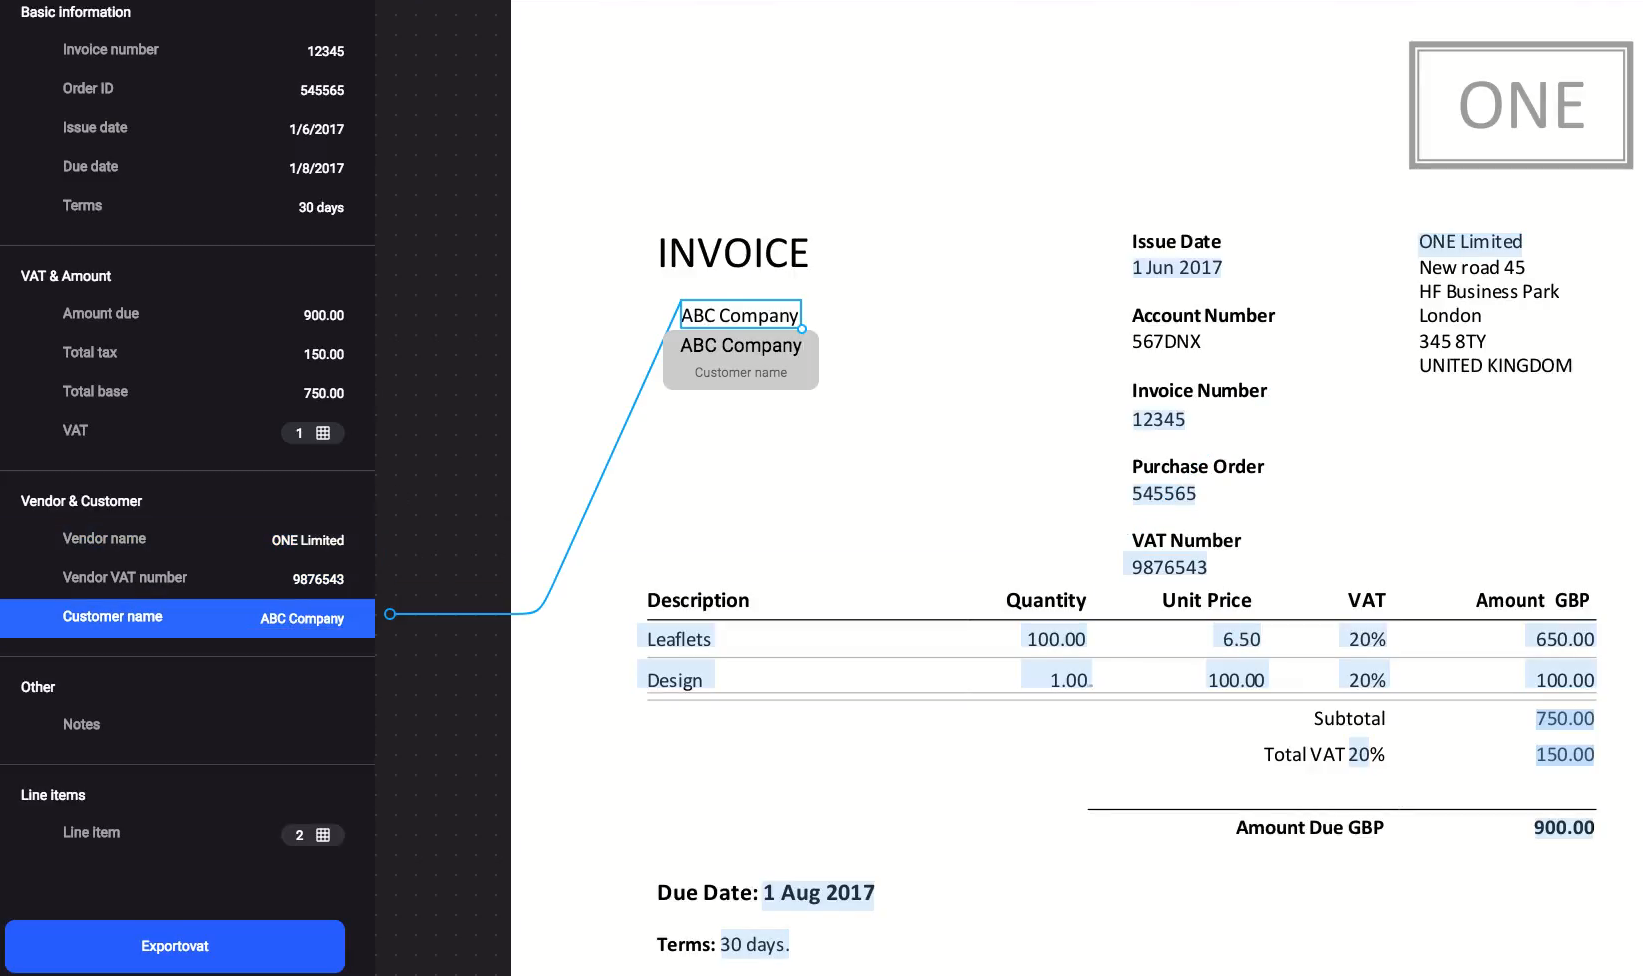
\includegraphics[width = 0.9\textwidth]{detection_structure_facture}
    \end{center}
    \caption{Analyse de la structure d'une facture avec correction manuelle possible, avec l'outil ELIS}
    \label{figure:detection_structure_facture}
\end{figure}
\FloatBarrier

\paragraph*{Détection automatique du document}
~\\

Lorsque l'on parle de détection automatique de la nature du document, on parle en fait de classification, l'utilisation d'une des méthodes décrites précédemment est donc tout à fait envisageable dans ce cas.

\paragraph*{Analyse de la structure du document}
~\\

Nous avons vu précédemment que traiter un document en tant qu'image était plus complexe que d'en extraire le texte brut.
Cela est vrai, mais le traitement en tant qu'image offre beaucoup plus de possibilités et n'entraîne aucune perte d'informations dans le processus.
Comme nous voulons ici analyser la structure du document, il faut le traiter sous sa forme initiale, sous forme d'image.
Pour réaliser cette analyse, il va donc être nécessaire d'utiliser des méthodes avancées d'apprentissage profond.

Comme précisé auparavant, ce sont les réseaux de neurones à convolution qui donne les meilleurs résultats concernant la reconnaissance d'images, la détection d'objet au sein d'une image et la segmentation d'images.
Ce que nous voulons réaliser s'apparente à une détection d'objet au sein d'une image, où les objets à détecter correspondent aux zones où se trouvent les informations à extraire.

Il existe plusieurs manières de détecter et identifier des objets.
Le système de détection YOLO (You Only Look Once) est actuellement le plus performant dans le domaine \cite{yolo}.
Il permet de gérer la détection d'objets au sein d'une image ainsi que leur classification, grâce à un réseau de neurones à convolution, en une seule étape.
Auparavant, il fallait utiliser deux réseaux de neurones à convolution, l'un pour détecter les limites des objets, l'autre pour classifier chaque objet détecté, un par un.
Le système YOLO est si efficient qu'il permet d'effectuer de la reconnaissance d'objets sur une vidéo en temps réel, à un rythme allant jusqu'à 45 images par secondes.

L'avantage de YOLO, qui pourrait permettre son fonctionnement dans notre cas, est qu'il identifie chaque objet en se basant sur l'image complète, ce qui lui permet de prendre en compte tout le contexte.
Pour comprendre qu'une zone spécifique d'un document est importante et savoir quelles informations on peut y trouver, il est nécessaire que le système considère le document dans sa globalité.

Les systèmes permettant la reconnaissance d'objets au sein d'une image ne sont pas pleinement adaptés à la reconnaissance de certaines zones d'un document.
L'adaptation du système YOLO à notre cas de figure nécessiterait donc une recherche approfondie du sujet.
Si l'adaptation est possible, le résultat serait donc un système permettant de détecter automatiquement  les zones du document à récupérer et de corréler chaque zone détectée avec le champ correspondant au sein de la base de données.

Une fois la détection et l'attribution des zones effectuée par le système, l'utilisateur doit avoir la main afin de pouvoir vérifier qu'elles sont bien placées et si ce n'est pas le cas, les déplacer manuellement.
Une correction effectuée par l'utilisateur aurait pour effet de venir en complément des données d'entraînement du système et ainsi lui permettre de s'adapter aux nouveaux documents.

\paragraph*{Lecture des informations et importation en base}
~\\

Une fois les zones détectées et attribuées aux champs de la base de données correspondants, l'étape restante est la lecture des informations, puis leur importation au sein de la base.
La lecture peut s'effectuer grâce à une méthode de reconnaissance optique de caractères.
Comme précisé auparavant, ces méthodes existent depuis un long moment et peuvent être mises en place en une simple ligne de code.
L'importation en base des informations ainsi extraites peut ensuite être effectuée.

\paragraph*{Conclusion}
~\\

Si l'on pouvait mettre en place un tel système au sein de \textsc{Sigma}, le travail de la comptabilité serait facilité.
Le temps actuellement passé à la saisie des données, ainsi qu'à la vérification des concordances entre les commandes et les factures serait énormément réduit.

Bien sûr, il faut garder à l'esprit qu'il a fallu une équipe de plus de 15 développeurs et experts en intelligence artificielle à la compagnie \textsc{Rossum} pour effectuer les recherches, puis développer un outil comparable.

\newpage
\subsection{Résumés de textes}

La synthèse de textes est un domaine qui se développe et qui est de plus en plus utilisé.
On peut noter, par exemple, l'apparition d'outils gratuits en ligne permettant de synthétiser des textes, par exemple <<~resoomer~>>, ou <<~autosummarizer~>>.
Il existe aussi des applications mobiles permettant de résumer des articles d'actualité, avec <<~inshorts~>>.
Synthétiser des textes automatiquement est utile et peut faire gagner énormément de temps à une personne et même à des compagnies dans leur globalité si les outils de synthèse utilisés sont performants et produisent des résumés entraînant le moins de perte d'information possible.

Pour tirer parti des méthodes de synthèses de textes d'un point de vue global sur une compagnie, on peut imaginer la mise en place d'un outil de synthèse accessible à tout moment au sein de l'ERP de l'entreprise.

Il y a trois types de synthèse possible~:~
\\
\begin{itemize}
    \item[\tiny$\bullet$] La synthèse par extraction extrait les phrases jugées les plus importantes du texte et les concatène pour produire un résumé.
    Cette méthode est très utilisée dans les systèmes réels.
    
    \item[\tiny$\bullet$] La synthèse par abstraction vise à résumer un texte en générant de nouvelles phrases à partir des informations importantes comprises dans le texte initial.
    Cette méthode permet de générer des résumés intelligents qui reprennent les informations utiles du texte dans sa globalité.
    Elle est peu mise en place dans les systèmes réels, de par sa complexité.
    
    \item[\tiny$\bullet$] La synthèse par compression de phrases consiste en la suppression des mots jugés superflus au sein des phrases.
    Elle peut aussi éliminer des phrases complètes si celles-ci ne sont pas jugées utiles.
\end{itemize}
~\\

De nombreux outils utilisant la synthèse par extraction, parfois liée à la compression de phrases, existent sur internet.
L'intérêt d'ajouter un outil réalisant la même tâche au sein d'un ERP a donc très peu d'intérêt.
Cependant, la synthèse par abstraction permet des résumés de bien meilleure qualité et il serait donc utile de mettre un tel outil à disposition des employés.

Lorsqu'il s'agit de traiter des problèmes concernant le traitement automatique du langage naturel, les modèles d'apprentissage profond généralement utilisés sont les RNN (<<~Recurrent Neural Network~>>, <<~réseaux de neurones récurrents~>>).
Les RNN sont un type de réseaux de neurones qui possède un cycle dans sa structure neuronale et qui sont capables de gérer des données d'entrées de taille variables et notamment des séquences.
Dans le cadre du traitement du langage naturel, les phrases correspondent à des suites de caractères, qui peuvent être considérées par un RNN comme des séquences.

Les RNN seuls ont beaucoup été utilisés dans la recherche sur le traitement du langage, mais des employés de \textsc{Google} ont développé un nouveau modèle en 2014, le <<~sequence to sequence model~>> \cite{seq2seq}, modèle de séquence à séquence.
Ce modèle est composé de deux parties qui se complètent~:~la première est un encodeur, la seconde est un décodeur.
Il s'agit de deux RNN différents qui sont combinés pour n'en former qu'un seul.

Le principe est le suivant~:~le rôle de l'encodeur est de comprendre la séquence donnée en entrée et de créer une représentation abstraite de celle-ci.
C'est comparable à un être humain qui comprend une phrase, celle-ci est représentée au sein du cerveau de manière abstraite, en tant que pensée, ce qui permet à ce dernier de la traiter plus facilement.

Cette représentation abstraite est ensuite donnée en entrée au décodeur, celui-ci va créer une nouvelle séquence correspondante aux données d'entrées.
Le fonctionnement est schématisé ci-dessous.

\FloatBarrier
\begin{figure}[h!]
    \begin{center}
        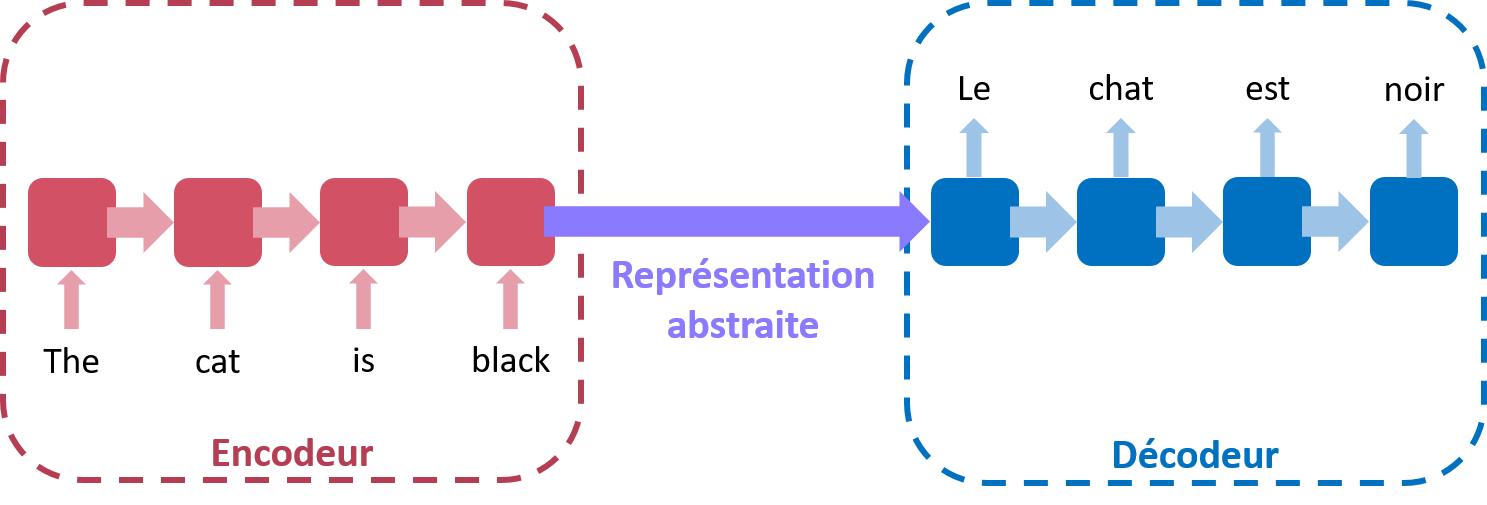
\includegraphics[width = 0.9\textwidth]{seq2seq}
    \end{center}
    \caption{Fonctionnement schématique d'un modèle de séquence à séquence}
    \label{figure:seq2seq}
\end{figure}
\FloatBarrier

Ce type de modèle a permis d'accélérer grandement la recherche dans le traitement du langage naturel et peut notamment être utilisé pour la synthèse de texte.
Correctement entraîné, un modèle de ce type est capable de comprendre les informations d'un texte qui ont une grande importance afin de les extraire grâce à l'encodeur.
Le décodeur est ensuite capable d'utiliser ces données importantes pour recréer des phrases dans un langage correct et compréhensible.
Le même modèle peut aussi être entraîné pour de la traduction automatique, par exemple.

Le principal problème que l'on pourrait rencontrer en développant un tel modèle est que son entraînement demande une grosse puissance de calcul.
Il faut donc une excellente machine pour effectuer l'entraînement de ce modèle.
En revanche, son utilisation demande peu de ressources, les machines des utilisateurs n'ont donc pas besoin d'être très performantes.

\newpage
\subsection{Gestion des stocks intelligente}

La gestion des stocks au sein d'une entreprise doit permettre de ne jamais manquer de quoi que ce soit, tout en faisant attention à ne pas trop acheter dans le souci d'économiser de l'argent.
Il faut constamment anticiper les besoins afin d'acheter au bon moment, ce qui n'est pas chose facile.
Dans cette section nous allons voir comment l'intelligence artificielle peut aider à simplifier la gestion des stocks des entreprises.

Dans de grandes compagnies qui doivent gérer des stocks immenses, il y a de plus en plus d'automatisation.
Par exemple, \textsc{Amazon} a automatisé, grâce à l'intelligence artificielle et des robots, la plupart des fonctions d'enlèvement/ramassage, d'emballage et de stockage.

\FloatBarrier
\begin{figure}[h!]
    \begin{minipage}[c]{0.55\textwidth}
        \begin{center}
            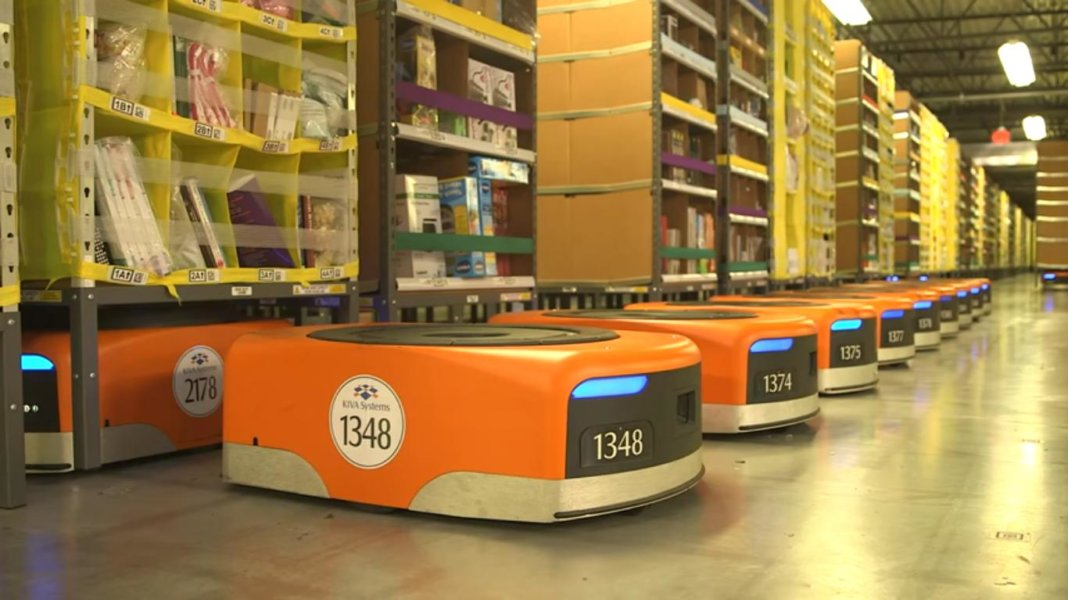
\includegraphics[width = 0.9\textwidth]{amazon}
        \end{center}
    \end{minipage}\hfill
    \begin{minipage}[c]{0.45\textwidth}
        \caption{Les robots Kiva d'\textsc{Amazon}}
        \label{figure:amazon}
    \end{minipage}
\end{figure}
\FloatBarrier

Des compagnies ont même poussé ce concept encore plus loin, créant des <<~entrepôts sans lumière~>>.
Comme \textsc{Siemens} qui possède des entrepôts capables de fonctionner dans le noir, de manière autonome, sans nécessiter le moindre être humain, et ce, pendant des semaines.
Ce genre d'entrepôts peut même permettre d'éliminer les besoins de climatisation ou de chauffage.

Dans des compagnies de taille moyenne, il est possible de mettre en place des systèmes capables d'anticiper les demandes de stocks à venir, et ainsi, pouvoir anticiper les achats nécessaires.

Pour réaliser de telles prédictions, les modèles les plus utilisés sont généralement des LSTM.
Un LSTM est un <<~long short-term memory~>>, c'est un réseau de neurones récurrents à mémoire court-terme et long terme.
C'est une version plus avancée d'un RNN qui convient mieux que ces derniers pour réaliser des prédictions.
Pour réaliser des prédictions solides, un tel modèle nécessite une quantité de données considérable, dans l'objectif de trouver des liens de cause à effet au sein de celles-ci.
Utiliser un tel système pour gérer les stocks au sein de \textsc{Disa} serait peu utile, car les données récoltées ne sont sûrement pas suffisantes.

\newpage
\subsection{Ordonnancement de phases de fabrication}

Lors de mon apprentissage au sein de \textsc{Disa}, il m'a été confié la tâche de développer un module sur \textsc{Sigma} permettant de planifier toutes les tâches de production.
La solution que j'ai développée n'est pas automatique, elle nécessite un travail manuel de placement de chaque phase par les responsables de production, dans cette section nous allons tenter de trouver une solution d'intelligence artificielle qui aurait pu me permettre d'automatiser ce processus.

Le problème se présente ainsi~:~on a une liste d'ordres de fabrication (OF) à réaliser.
Chacun possède une date de mise à disposition.
Le but est évidemment de finir la production complète de l'OF avant celle-ci.
Chaque OF est composé d'une liste de phases de fabrication qui doivent être réalisées sur des machines qui leur sont dédiées.
Il faut donc organiser sur un planning toutes les phases de fabrication sur leur machine, le tout en prenant en compte un ordre de priorité sur les OF dont la date de mise à disposition est proche.

Pour simplifier, on peut poser une liste de contraintes que les solutions devront respecter pour être valables.
\\
\begin{itemize}
    \item[\tiny$\bullet$] Les phases doivent être ordonnancées sur les machines qui permettent leur fabrication.
    \item[\tiny$\bullet$] Les phases ne peuvent pas se chevaucher sur une même machine.
    \item[\tiny$\bullet$] Les phases d'un même ordre de fabrication doivent être réalisées dans l'ordre.
    \item[\tiny$\bullet$] Pour commencer une phase, la précédente doit être terminée.
    \item[\tiny$\bullet$] Toutes les phases doivent être incluses au sein de l'ordonnancement.
\end{itemize}
~\\

Après de longues recherches, la solution relevant de l'intelligence artificielle semblant de loin la mieux adaptée à un problème d'ordonnancement est l'utilisation d'un algorithme génétique.

Les algorithmes génétiques permettent de proposer des solutions à un problème en utilisant une simulation du concept de la sélection naturelle (voir la section \ref{section:ga} pour plus de détails).
Comme il n'y a pas qu'une seule solution possible à un problème d'ordonnancement, l'utilisation de cette méthode pourrait être très efficace.

L'idée serait donc de générer une population de manière pseudo-aléatoire, en s'assurant que chaque solution de cette population prenne en compte les contraintes définies précédemment.

Les solutions de cette population ayant le plus de chances de se reproduire seraient celles avec un ordonnancement des phases laissant le moins de temps libre possible aux machines.
Ainsi, en laissant tourner l'algorithme génétique et en s'assurant que toutes les solutions générées respectent les contraintes définies, on obtiendrait, à terme, un ensemble de solutions valables.
Ces solutions peuvent être proposées au responsable de la production afin qu'il en sélectionne une qui lui convient.

Le planning de fabrication pourrait alors être automatiquement mis à jour avec l'ordonnancement de phases choisi.
Ce fonctionnement pourrait bien entendu être généralisé pour un usage en dehors du contexte de \textsc{Disa}.

L'ordonnancement de tâches par l'intelligence artificielle est un domaine pour le moment très peu exploré.
L'ordonnancement par des réseaux de neurones pourrait être un domaine de recherche intéressant, puisqu'aucune recherche ne semble avoir été menée sur ce sujet pour le moment \cite{ordo}.

\newpage
\subsection{Assistant intelligent permettant d'aider les utilisateurs au quotidien}

Afin d'aider les utilisateurs dans leur utilisation d'un ERP on pourrait imaginer un système d'assistant qui serait présent pour faciliter les saisies d'informations et jouer un rôle d'anticipation tel que le ferait un assistant comme \textsc{Google Home} ou \textsc{Alexa} d'\textsc{Amazon}.
L'idée serait de pouvoir <<~communiquer~>> à l'oral ou à l'écrit avec l'ERP.
On pourrait ainsi demander des informations à l'assistant telles que l'état des stocks d'un article, le statut actuel de différentes phases de fabrication, etc.

Un tel outil permettrait de faciliter les interactions entre l'utilisateur et l'ERP.
Actuellement, lorsque l'on souhaite accéder à des informations sur n'importe quelle application il est nécessaire de naviguer soi-même jusqu'aux informations voulues.
L'intérêt de l'assistant serait justement de naviguer automatiquement jusqu'aux informations, à partir d'une demande verbale.
L'utilisation d'un tel assistant mènerait donc à un gain de temps certain au quotidien.

La société \textsc{Avaamo}, spécialisée dans le développement d'assistants intelligents, a présenté un assistant permettant de faciliter l'accessibilité à l'ERP SAP \cite{assistant}.

On peut imaginer que dans un futur proche, ce genre d'assistants soient intégrés par défaut au sein de beaucoup d'ERP, au même titre que les assistants intelligents sur les smartphones.
